%!TEX root = slides.tex

\section{Bayesian Population Pharmacodynamic Modeling}

\subsection{Recommended References}
\begin{frame}{Bayesian Population Pharmacokinetic Modeling - Recommended References}
    \begin{vfilleditems}
        \item \textcite{Gabrielsson2006PKPDbook}:
        \begin{vfilleditems}
            \item Chapter 1: General Principles
            \item Chapter 3: Pharmacodynamic Concepts
        \end{vfilleditems}
        \item \textcite{Owen2014PKPDbook}:
        \begin{vfilleditems}
            \item Chapter 10: PK/PD Models
        \end{vfilleditems}
        \item \textcite{Bonate2011PKPDbook}:
        \begin{vfilleditems}
            \item Chapter 10: Bayesian Modeling regression
        \end{vfilleditems}
        \item \textcite{margossian2022torsten}
    \end{vfilleditems}
\end{frame}

\subsection{Pharmacodynamics}
\begin{frame}{Pharmacodynamics}
    \begin{defn}[Pharmacodynamics]
        \begin{quotation}
            Pharmacodynamics can be defined as the study of the time course of the
            biological effects of drugs, the relationship of the effects to drug exposure,
            and the mechanisms of drug action.
        \end{quotation}
        \vfill \vfill
        \textcite[199]{Gabrielsson2006PKPDbook}
    \end{defn}
\end{frame}

\begin{frame}{Pharmacodynamics}
    Pharmacodynamics is generally represented as \textbf{``PD'' compartments} in a model.
    \vfill
    They can be either:
    \begin{vfilleditems}
        \item \textbf{Pharmacodynamic} (PD) models with only PD compartments
        \item \textbf{Phamacokynetic-Pharmacodynamic} (PKPD) models with both PK compartments and PD compartments
    \end{vfilleditems}
\end{frame}

\subsection{Compartment Models}
\begin{frame}{PD Compartment Models}
    There are several ways to specify (and characterize) PD compartmental models.
    \vfill
    Here we'll use the following characterization for the PD compartments:
    \begin{vfilleditems}
        \item \textbf{Impact}:
        \begin{vfilleditems}
            \item Production Rate
            \item Degradation Rate
        \end{vfilleditems}
        \item \textbf{Rate}:
        \begin{vfilleditems}
            \item Stimulation
            \item Inhibition
        \end{vfilleditems}
        \item \textbf{Effect}:
        \begin{vfilleditems}
            \item Emax
            \item Linear
            \item Sigmoid
            \item $\ldots$
        \end{vfilleditems}
    \end{vfilleditems}
\end{frame}

\begin{frame}{PD Compartment Models}
    $$
        \text{Resp}^{\prime} = \text{Resp}_0 \cdot k_{\text{out}} \cdot \operatorname{Impact}(\operatorname{Rate}, \operatorname{Effect}, \text{PK compartment}) - k_{\text{out}} \cdot \text{Resp}
    $$
    \vfill
    Example with Production Rate, Stimulation, Emax and Central PK compartment:
    $$
        \text{Resp}^{\prime} = \text{Resp}_0 \cdot k_{\text{out}} \cdot \left(1 + \frac{\text{Emax} * \text{Central}}{\text{EC}_{50} + \text{Central}} \right) - k_{\text{out}} \cdot \text{Resp}
    $$
\end{frame}

\subsection{Bayesian PD Models}
\begin{frame}{How to make it Bayesian?}
    Just put \textbf{priors} in all parameters:
    $$
        \begin{aligned}
            k_{\text{out}} & \sim \text{LogNormal}(\log{\mu_{k_{\text{out}}}}, \sigma_{k_{\text{out}}}) \\
            \text{Resp}_0  & \sim \text{LogNormal}(\log{\mu_{\text{Resp}_0}}, \sigma_{\text{Resp}_0})   \\
            \ldots
        \end{aligned}
    $$
\end{frame}

\subsection{Bayesian PopPD Models}
\begin{frame}{How to make it Bayesian?}
    Just put \textbf{priors} in all parameters:
    $$
        \begin{aligned}
            \theta   & \sim \text{Normal}(0, 2.5)  \\
            \omega   & \sim \text{Normal}^+(0, 2.5)  \\
            \eta_{i} & \sim \text{Normal}(0, \omega)
        \end{aligned}
    $$
    \vfill
    where each subject $i$ has its own $\eta_i$.
\end{frame}

\begin{frame}{Example}
    \centering
    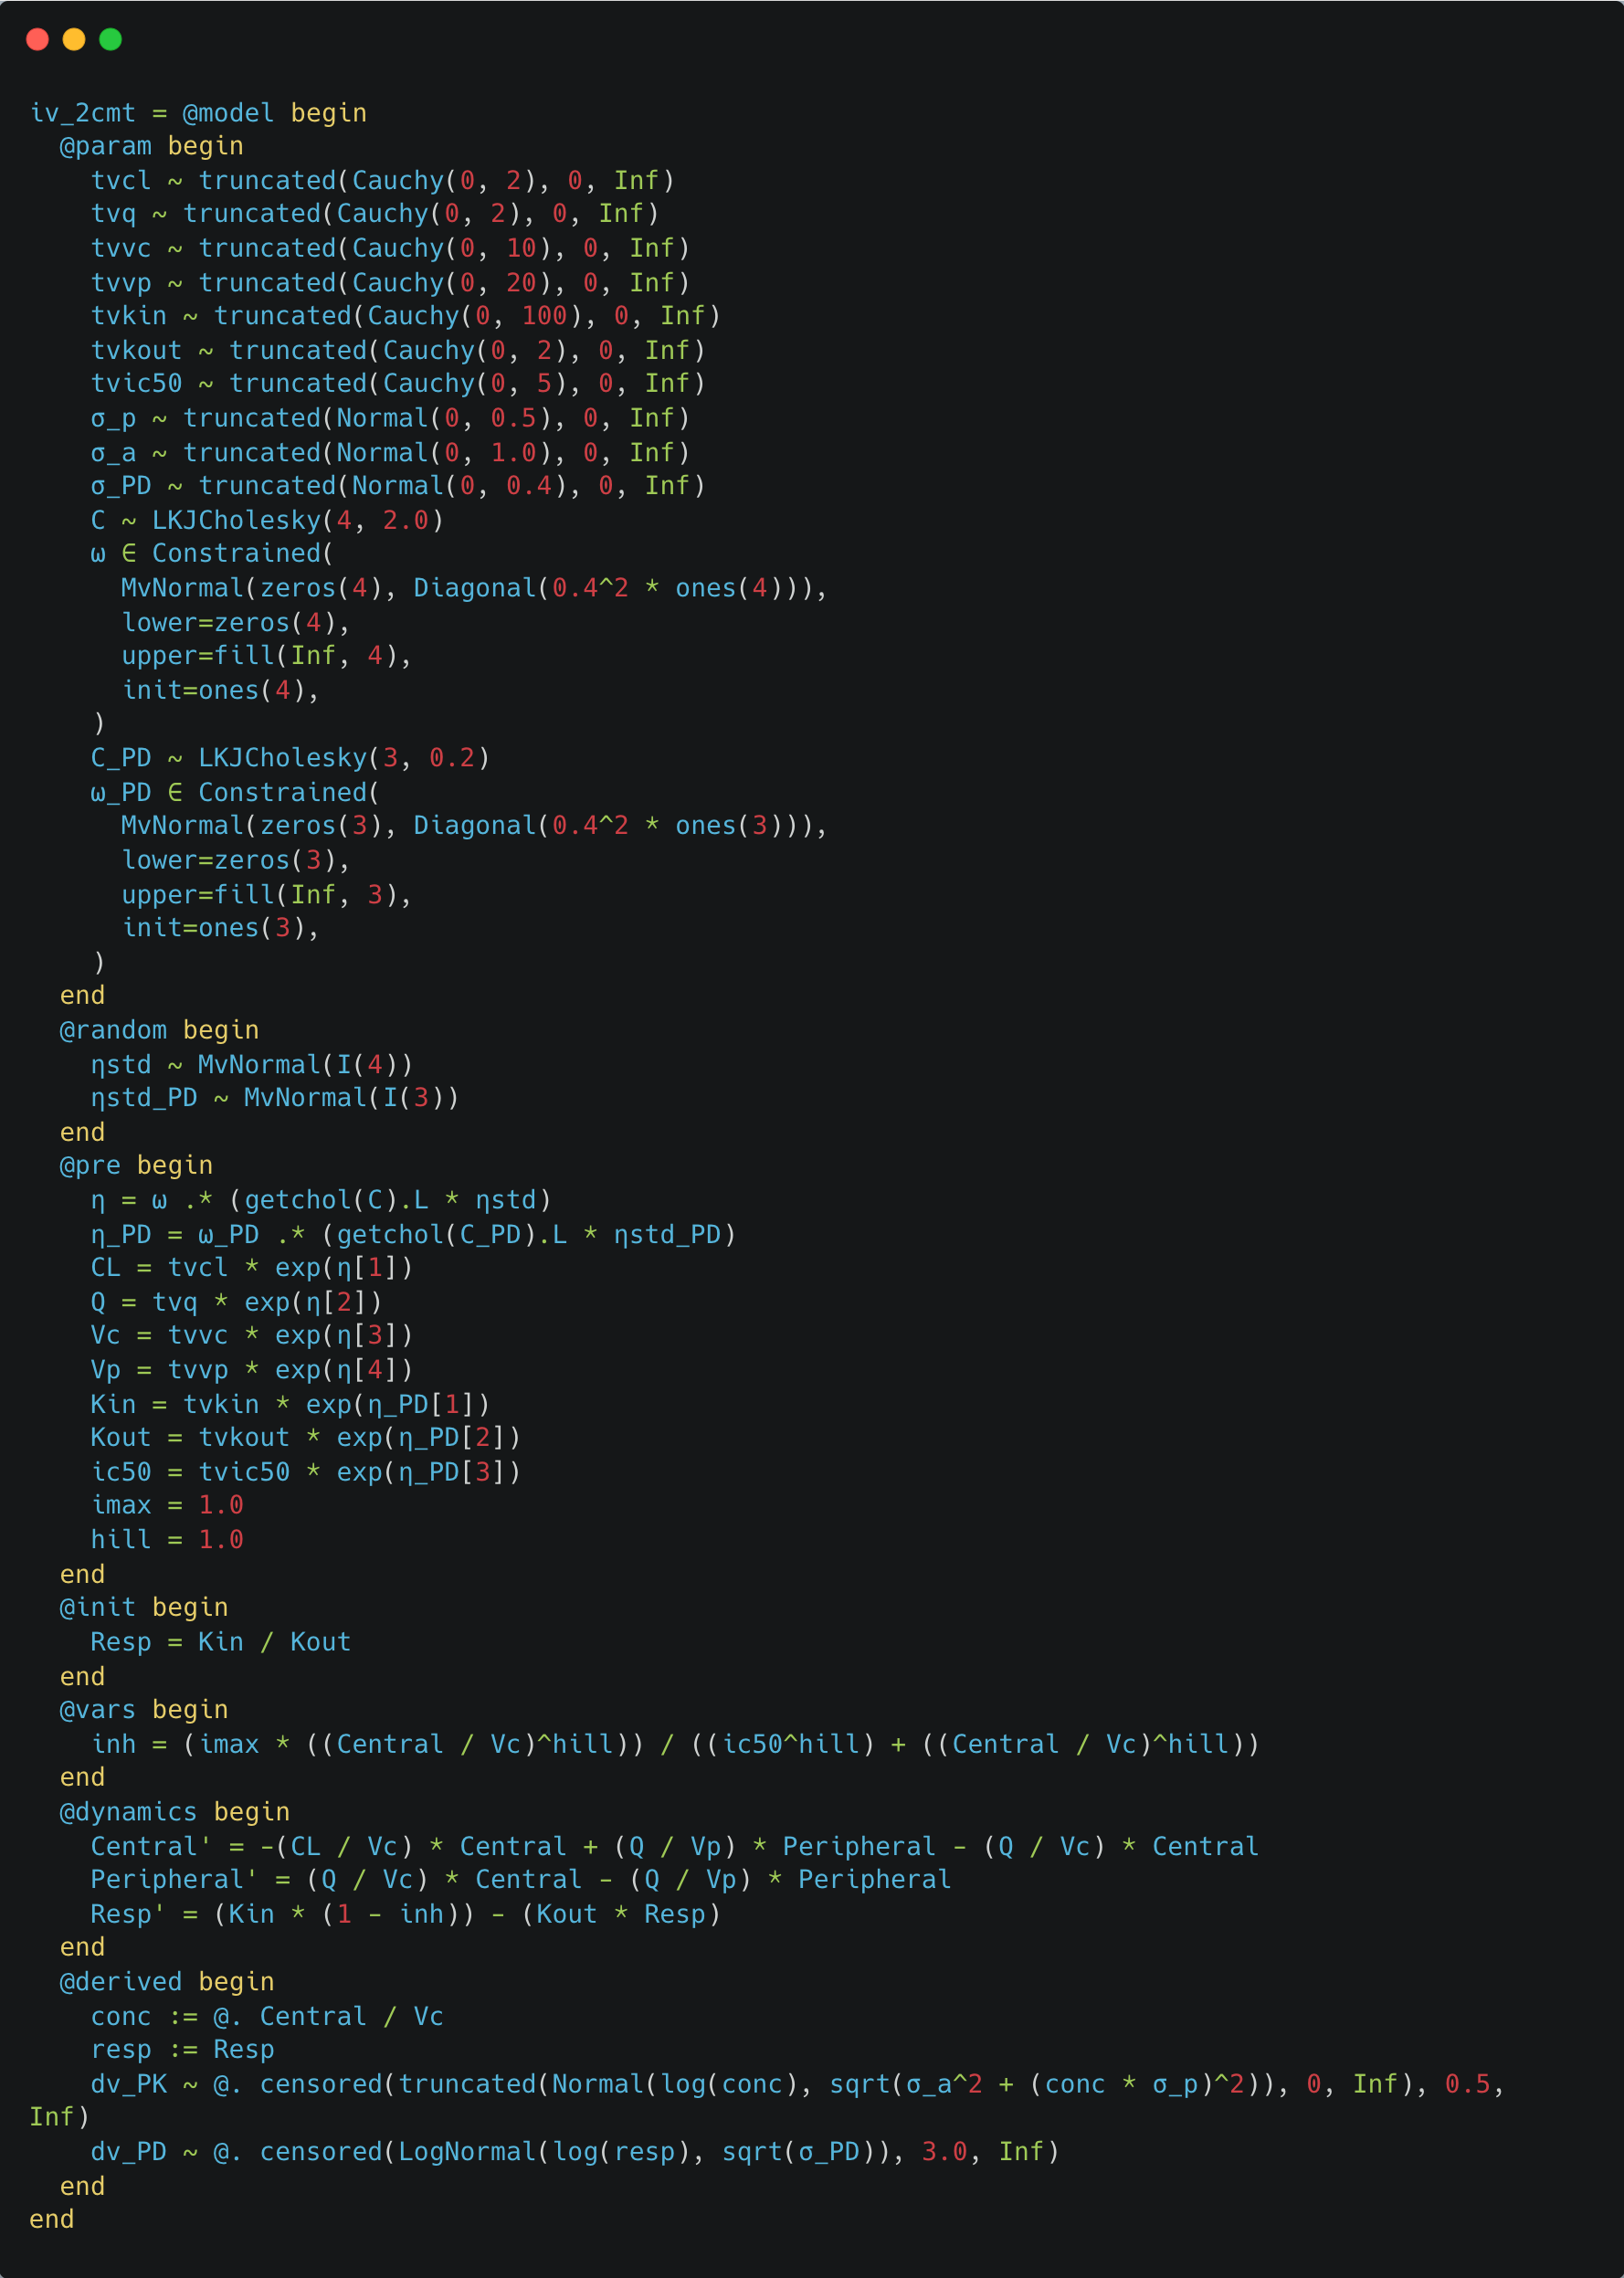
\includegraphics[width=0.3\columnwidth]{pkpd.png}
\end{frame}
